\documentclass{standalone}
\usepackage{tikz}
\usetikzlibrary{patterns, positioning}

\begin{document}
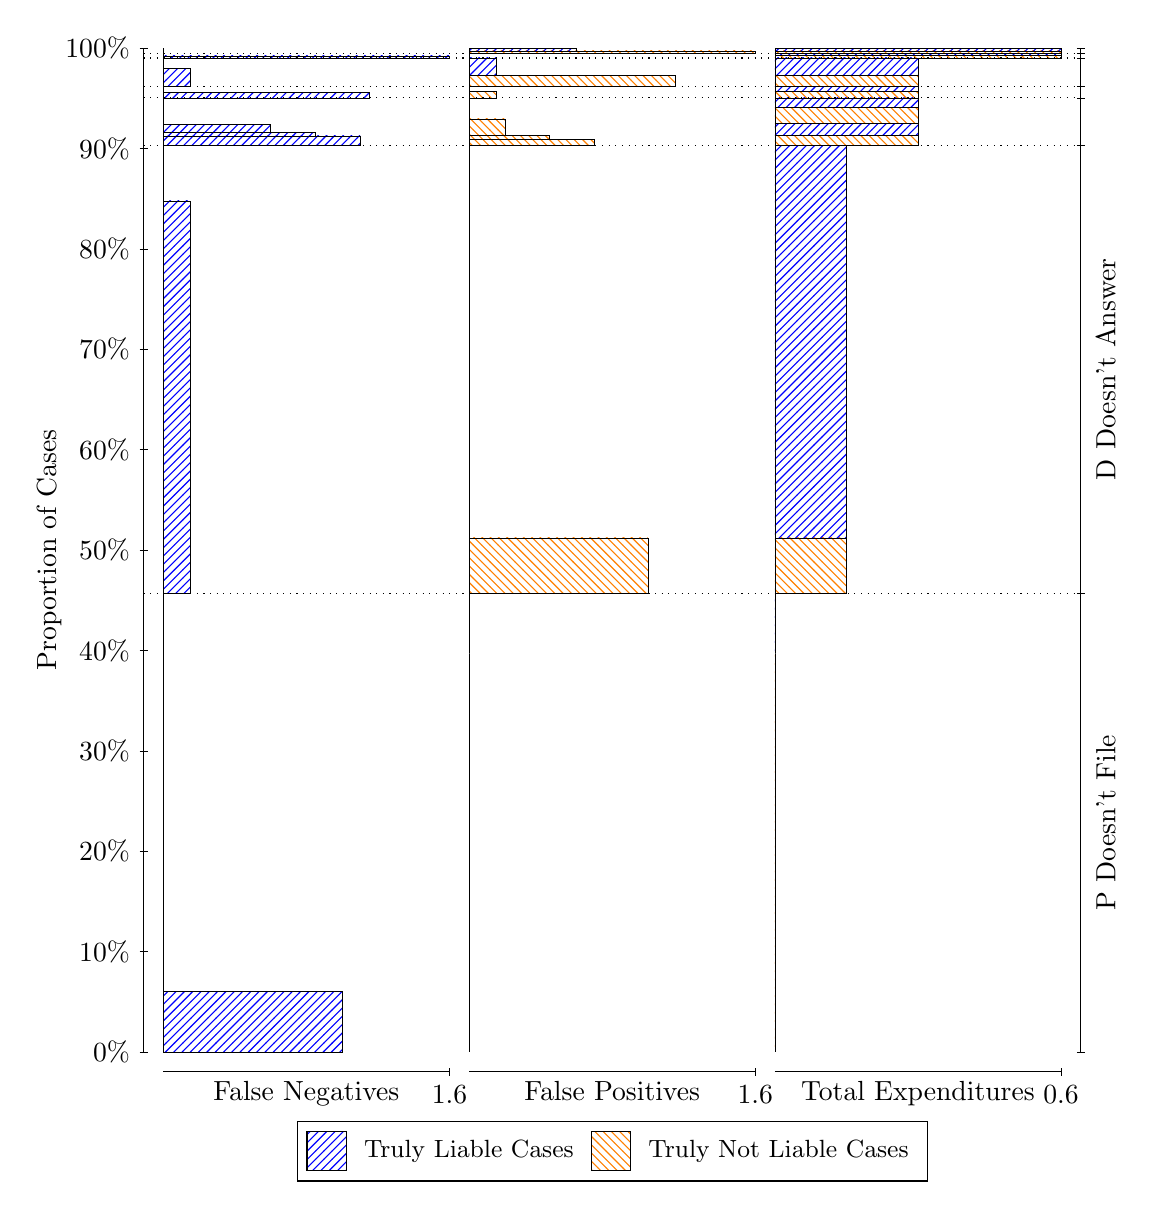
\begin{tikzpicture}
\draw[black, very thin] (1.5,1.75) -- (1.5,14.5);
\node[rotate=90, anchor=center] at (0.3, 8.125) {Proportion of Cases};
\draw[black, very thin] (1.45,1.75) -- (1.55,1.75);
\node[anchor=east] at (1.45, 1.75) {0\%};
\draw[black, very thin] (1.45,3.025) -- (1.55,3.025);
\node[anchor=east] at (1.45, 3.025) {10\%};
\draw[black, very thin] (1.45,4.3) -- (1.55,4.3);
\node[anchor=east] at (1.45, 4.3) {20\%};
\draw[black, very thin] (1.45,5.575) -- (1.55,5.575);
\node[anchor=east] at (1.45, 5.575) {30\%};
\draw[black, very thin] (1.45,6.85) -- (1.55,6.85);
\node[anchor=east] at (1.45, 6.85) {40\%};
\draw[black, very thin] (1.45,8.125) -- (1.55,8.125);
\node[anchor=east] at (1.45, 8.125) {50\%};
\draw[black, very thin] (1.45,9.4) -- (1.55,9.4);
\node[anchor=east] at (1.45, 9.4) {60\%};
\draw[black, very thin] (1.45,10.675) -- (1.55,10.675);
\node[anchor=east] at (1.45, 10.675) {70\%};
\draw[black, very thin] (1.45,11.95) -- (1.55,11.95);
\node[anchor=east] at (1.45, 11.95) {80\%};
\draw[black, very thin] (1.45,13.225) -- (1.55,13.225);
\node[anchor=east] at (1.45, 13.225) {90\%};
\draw[black, very thin] (1.45,14.5) -- (1.55,14.5);
\node[anchor=east] at (1.45, 14.5) {100\%};

\draw[black, very thin] (13.4,1.75) -- (13.4,14.5);
\draw[black, very thin] (13.35,1.75) -- (13.45,1.75);
\node[anchor=west] at (13.35, 1.75) {};
\draw[black, very thin] (13.35,7.5747) -- (13.45,7.5747);
\node[anchor=west] at (13.35, 7.5747) {};
\draw[black, very thin] (13.35,13.265) -- (13.45,13.265);
\node[anchor=west] at (13.35, 13.265) {};
\draw[black, very thin] (13.35,13.868) -- (13.45,13.868);
\node[anchor=west] at (13.35, 13.868) {};
\draw[black, very thin] (13.35,14.016) -- (13.45,14.016);
\node[anchor=west] at (13.35, 14.016) {};
\draw[black, very thin] (13.35,14.374) -- (13.45,14.374);
\node[anchor=west] at (13.35, 14.374) {};
\draw[black, very thin] (13.35,14.435) -- (13.45,14.435);
\node[anchor=west] at (13.35, 14.435) {};
\draw[black, very thin] (13.35,14.5) -- (13.45,14.5);
\node[anchor=west] at (13.35, 14.5) {};

\draw[black, very thin, pattern color=blue, pattern=north east lines] (1.75,1.75) rectangle (4.0208,2.5162);
\draw[black, very thin, pattern color=orange, pattern=north west lines] (1.75,2.5162) rectangle (1.75,7.5747);
\draw[black, very thin, pattern color=blue, pattern=north east lines] (1.75,7.5747) rectangle (2.0906,12.56);
\draw[black, very thin, pattern color=orange, pattern=north west lines] (1.75,12.56) rectangle (1.75,13.265);
\draw[black, very thin, pattern color=blue, pattern=north east lines] (1.75,13.265) rectangle (4.2479,13.383);
\draw[black, very thin, pattern color=blue, pattern=north east lines] (1.75,13.383) rectangle (3.6802,13.427);
\draw[black, very thin, pattern color=blue, pattern=north east lines] (1.75,13.427) rectangle (3.1125,13.533);
\draw[black, very thin, pattern color=orange, pattern=north west lines] (1.75,13.533) rectangle (1.75,13.868);
\draw[black, very thin, pattern color=blue, pattern=north east lines] (1.75,13.868) rectangle (4.3615,13.934);
\draw[black, very thin, pattern color=orange, pattern=north west lines] (1.75,13.934) rectangle (1.75,14.016);
\draw[black, very thin, pattern color=blue, pattern=north east lines] (1.75,14.016) rectangle (2.0906,14.242);
\draw[black, very thin, pattern color=orange, pattern=north west lines] (1.75,14.242) rectangle (1.75,14.374);
\draw[black, very thin, pattern color=blue, pattern=north east lines] (1.75,14.374) rectangle (5.3833,14.4);
\draw[black, very thin, pattern color=orange, pattern=north west lines] (1.75,14.4) rectangle (1.75,14.435);
\draw[black, very thin, pattern color=orange, pattern=north west lines] (1.75,14.435) rectangle (1.75,14.463);
\draw[black, very thin, pattern color=blue, pattern=north east lines] (1.75,14.463) rectangle (1.75,14.5);
\draw[black, very thin, pattern color=orange, pattern=north west lines] (5.6333,1.75) rectangle (5.6333,6.8085);
\draw[black, very thin, pattern color=blue, pattern=north east lines] (5.6333,6.8085) rectangle (5.6333,7.5747);
\draw[black, very thin, pattern color=orange, pattern=north west lines] (5.6333,7.5747) rectangle (7.9042,8.2794);
\draw[black, very thin, pattern color=blue, pattern=north east lines] (5.6333,8.2794) rectangle (5.6333,13.265);
\draw[black, very thin, pattern color=orange, pattern=north west lines] (5.6333,13.265) rectangle (7.2229,13.341);
\draw[black, very thin, pattern color=orange, pattern=north west lines] (5.6333,13.341) rectangle (6.6552,13.394);
\draw[black, very thin, pattern color=orange, pattern=north west lines] (5.6333,13.394) rectangle (6.0875,13.6);
\draw[black, very thin, pattern color=blue, pattern=north east lines] (5.6333,13.6) rectangle (5.6333,13.868);
\draw[black, very thin, pattern color=orange, pattern=north west lines] (5.6333,13.868) rectangle (5.974,13.95);
\draw[black, very thin, pattern color=blue, pattern=north east lines] (5.6333,13.95) rectangle (5.6333,14.016);
\draw[black, very thin, pattern color=orange, pattern=north west lines] (5.6333,14.016) rectangle (8.2448,14.149);
\draw[black, very thin, pattern color=blue, pattern=north east lines] (5.6333,14.149) rectangle (5.974,14.374);
\draw[black, very thin, pattern color=orange, pattern=north west lines] (5.6333,14.374) rectangle (5.6333,14.409);
\draw[black, very thin, pattern color=blue, pattern=north east lines] (5.6333,14.409) rectangle (5.6333,14.435);
\draw[black, very thin, pattern color=orange, pattern=north west lines] (5.6333,14.435) rectangle (9.2667,14.463);
\draw[black, very thin, pattern color=blue, pattern=north east lines] (5.6333,14.463) rectangle (6.9958,14.5);
\draw[black, very thin, pattern color=orange, pattern=north west lines] (9.5167,1.75) rectangle (9.5167,6.8085);
\draw[black, very thin, pattern color=blue, pattern=north east lines] (9.5167,6.8085) rectangle (9.5167,7.5747);
\draw[black, very thin, pattern color=orange, pattern=north west lines] (9.5167,7.5747) rectangle (10.425,8.2794);
\draw[black, very thin, pattern color=blue, pattern=north east lines] (9.5167,8.2794) rectangle (10.425,13.265);
\draw[black, very thin, pattern color=orange, pattern=north west lines] (9.5167,13.265) rectangle (11.333,13.394);
\draw[black, very thin, pattern color=blue, pattern=north east lines] (9.5167,13.394) rectangle (11.333,13.543);
\draw[black, very thin, pattern color=orange, pattern=north west lines] (9.5167,13.543) rectangle (11.333,13.75);
\draw[black, very thin, pattern color=blue, pattern=north east lines] (9.5167,13.75) rectangle (11.333,13.868);
\draw[black, very thin, pattern color=orange, pattern=north west lines] (9.5167,13.868) rectangle (11.333,13.95);
\draw[black, very thin, pattern color=blue, pattern=north east lines] (9.5167,13.95) rectangle (11.333,14.016);
\draw[black, very thin, pattern color=orange, pattern=north west lines] (9.5167,14.016) rectangle (11.333,14.149);
\draw[black, very thin, pattern color=blue, pattern=north east lines] (9.5167,14.149) rectangle (11.333,14.374);
\draw[black, very thin, pattern color=orange, pattern=north west lines] (9.5167,14.374) rectangle (13.15,14.409);
\draw[black, very thin, pattern color=blue, pattern=north east lines] (9.5167,14.409) rectangle (13.15,14.435);
\draw[black, very thin, pattern color=orange, pattern=north west lines] (9.5167,14.435) rectangle (13.15,14.463);
\draw[black, very thin, pattern color=blue, pattern=north east lines] (9.5167,14.463) rectangle (13.15,14.5);
\draw[black, dotted] (1.5,7.5747) -- (13.4,7.5747);
\draw[black, dotted] (1.5,13.265) -- (13.4,13.265);
\draw[black, dotted] (1.5,13.868) -- (13.4,13.868);
\draw[black, dotted] (1.5,14.016) -- (13.4,14.016);
\draw[black, dotted] (1.5,14.374) -- (13.4,14.374);
\draw[black, dotted] (1.5,14.435) -- (13.4,14.435);
\draw[black, very thin] (1.75,1.5) -- (5.3833,1.5);
\node[anchor=north] at (3.5667, 1.5) {False Negatives};
\draw[black, very thin] (5.3833,1.45) -- (5.3833,1.55);
\node[anchor=north] at (5.3833, 1.45) {1.6};

\draw[black, very thin] (5.6333,1.5) -- (9.2667,1.5);
\node[anchor=north] at (7.45, 1.5) {False Positives};
\draw[black, very thin] (9.2667,1.45) -- (9.2667,1.55);
\node[anchor=north] at (9.2667, 1.45) {1.6};

\draw[black, very thin] (9.5167,1.5) -- (13.15,1.5);
\node[anchor=north] at (11.333, 1.5) {Total Expenditures};
\draw[black, very thin] (13.15,1.45) -- (13.15,1.55);
\node[anchor=north] at (13.15, 1.45) {0.6};

\node[black, centered, rotate=90] at (13.72, 4.6623) {P Doesn't File};
\node[black, centered, rotate=90] at (13.72, 10.42) {D Doesn't Answer};






\draw (7.449999999999999,1.5) node[draw=none] (baseCoordinate) {};
\begin{scope}[align=center]
        \matrix[scale=0.5, draw=black, below=0.5cm of baseCoordinate, nodes={draw}, column sep=0.1cm]{
            \node[rectangle, draw, minimum width=0.5cm, minimum height=0.5cm, pattern=north east lines, pattern color=blue] {}; &
            \node[draw=none, font=\small] (B) {Truly Liable Cases}; &
            \node[rectangle, draw, minimum width=0.5cm, minimum height=0.5cm, pattern=north west lines, pattern color=orange] {}; &
            \node[draw=none, font=\small] (B) {Truly Not Liable Cases}; \\
            };
\end{scope}

\end{tikzpicture}
\end{document}